\documentclass[authoryear,preprint,review,10pt]{elsarticle}
\usepackage{amssymb,amsthm,amsmath,setspace}
\usepackage{url,color}
\usepackage{lineno}
%\usepackage[labelfont=bf,format=hang,textfont=it]{caption}
\usepackage{graphicx}
\usepackage{microtype}
\usepackage[letterpaper,text={15cm,23cm}]{geometry}
\usepackage{natbib}
\usepackage{hyperref}

%% for internal use
\newcommand{\fixme}[1]{\emph{\marginpar{FIXME} (#1)}}
\newcommand{\readme}[1]{\emph{\marginpar{README} (#1)}}

\definecolor{Red}{rgb}{0.5,0,0}
\definecolor{Blue}{rgb}{0,0,0.5}
\hypersetup{%
  pdftitle = {Real-time change detection},
  pdfsubject = {},
  pdfkeywords = {monitoring, time series, MODIS, NDVI},
  pdfauthor = {Jan Verbesselt, Achim Zeileis},
  %% change colorlinks to false for pretty printing
  colorlinks = {true},
  linkcolor = {Blue},
  citecolor = {Blue},
  urlcolor = {Red},
  hyperindex = {true},
  linktocpage = {true},
}


\journal{Remote Sensing of Environment}

\begin{document}
%% \linenumbers
\begin{frontmatter}

    \title
    {
    Real-time land cover disturbance detection \\ using satellite image time series
    %real-time change detection using satellite image time series:
    %Early warning for forest disturbances
    % Real-time change detection of forest disturbances using satellite image time series
    }
    \author[WUR]{Jan Verbesselt\corref{cor}}
    \ead{Jan.Verbesselt@wur.nl}
    \author[UIBK]{Achim Zeileis}
    \ead{Achim.Zeileis@R-project.org}
    \author[WUR]{Martin Herold}
    \ead{Martin.Herold@wur.nl}
    \cortext[cor]{Corresponding author.}
    \address[WUR]{Remote Sensing Team, Wageningen University, \\
           Droevendaalsesteeg 3, Wageningen 6708 PB, The Netherlands}
    \address[UIBK]{Department of Statistics, Universit\"at Innsbruck \\
           Universit\"atsstr.~15, A-6020 Innsbruck, Austria}

\singlespace

\begin{abstract}

% satellite image time series are faster and faster available - methods to deal with this are lacking
Real-time monitoring forest and land cover disturbances are critical for addressing impacts on carbon storage, biodiversity, and socio-ecological processes. Satellite remote sensing enables cost-effective and accurate monitoring at frequent time steps over large areas. Yet, methods to detect changes in real-time within newly captured satellite images are urgently needed. 

We are proposing a time series analysis approach to detect disturbances in real-time, i.e. when new satellite images are being captured. A stable history period is selected to model normal expected behaviour and enable differentiation between normal an abnormal changes occurring with recently captured satellite images.

%We are proposing a generic approach to detect disturbances in real-time 
%based on time series modelling of the stable historical period, representing expected normal behaviour. As such,
%the differentiation between normal and abnormal change in real-time becomes
%possible when new data is captured. 

Validation and accuracy assessment of the real-time change detection method is done by 
(1)~simulating 16-day MODIS NDVI time series (2000--2010) with different amount of noise, seasonality and containing
disturbances at the end of the time series, (2)~using real MODIS satellite image time series. 

Results illustrate that abrupt changes at the end of time series are
successfully detected while being robust for strong seasonality and noise. 

The signal-to-noise ratio of the time series being analysed for real-time change remains the most important driver of accuracy and potential to detect changes.
As such, data pre-processing in order to improve the quality and reliability of remotely sensed time series remains essential to enable change detection in time series data. 

The method is publicly available within the BFAST package for R. This method is specifically developed so that it can be used a global scale since is fast, does not
depend on thresholds or change type definitions and does not require gap filling of time series (e.g. clouds). Furthermore,
the method is flexible and can be applied for different purposes (e.g. fire or oil spill detection) and onto all sorts of time series data (e.g. in-situ monitoring sensors or different types of satellite data such as the DMCii satellite image time series).

\textbf{Research Highlights}
\begin{itemize}
    \item Real-time change detection within newly measured data using time series analysis
    \item A new method is proposed is freely available as a function in the BFAST package for open source R software
    \item The method is validated by simulating time series and applying it on real satellite data
    \item The approach is robust, fast and flexible to different data sets and does not require gap filling
\end{itemize}

\end{abstract}

\begin{keyword}
Early warning \sep real-time \sep change detection \sep land cover and land use change\sep disturbance \sep NDVI \sep time series \sep MODIS \sep vegetation dynamics \sep phenology
\end{keyword}

\end{frontmatter} 

\section{Introduction}

% forest disturbances and their importance
% the importance of detecting disturbances in real-time? Disaster monitoring/ fast detection of current forest cover changes/ etc.

Real-time forest and land cover disturbance monitoring is critical for tracking human-induced and natural disturbances promptly. Such information is needed for signalling abnormal developments, quickly raising awareness, and allow for prompt actions to intervene, relief efforts and reduce negative impacts to natural resources, humans, and infrastructure. Real-time remote sensing approaches are already performed for weather monitoring and prediction \citep{Ebert:2007tj}, and in case of after-disasters and relief efforts \citep{Tralli:2005ch}. However, key to approaches looking at forest and land cover disturbances is that many change events occur worldwide at unknown locations with unknown change magnitudes. In this sense, remote sensing tools can be in the first instance used to alert when things start to appear \emph{abnormal}. For example, deviations from \emph{normal} land surface phenology, defined as the seasonal variation in vegetated land surface from remote sensing \citep{White2009}, can indicate important changes forest health \citep{Stone2008,Morisette2009}, carbon status, and even climate change \citep{Cleland2007,Hargrove2009}.

% satellite data
Satellite sensors are well-suited to provide consistent and frequent
measurements over large areas which is appropriate for capturing the effects
of many processes that cause change, including natural (e.g., insect attacks, droughts, fires, floods) and
anthropogenic (e.g., deforestation, urbanisation, farming) disturbances
\citep{Jin2005}. % different change types in ecosystem dynamics
Many types of changes affecting the land surface and land cover operate in ecosystems and range from diurnal cycles to long-term change in vegetation patterns. The ecosystem changes commonly observed with remote sensing approaches can be divided into three categories: (1)~\emph{seasonal or cyclic change}, driven by annual temperature and rainfall interactions impacting plant phenology resulting in distinct intra-annual patterns for different vegetation types; (2)~\emph{gradual trend change} such as trends in mean annual rainfall or gradual change in land management (e.g. forest regrowth after fire) that result in changes over several years or decades; and (3)~\emph{abrupt trend change}, caused by events from human activities (e.g. deforestation) or natural causes (e.g. wind throw) that change land cover over short time frames (days or weeks). %These different types of changes commonly operate in parallel and approaches to detect and map a particular change type have to include information about the other types to avoid confusion and wrong labelling of change. 

% problem statement
Estimating change from remotely sensed data is not straightforward, since time
series contain a combination of seasonal, gradual and abrupt ecosystem changes occurring in parallel,
in addition to noise that originates from the sensing environment (e.g., view
angle), remnant geometric errors, atmospheric scatter and cloud effects
\citep{deBeurs:2005jq, Beurs2005a, Roy2002, Wolfe1998}. The ability of any system to detect change depends on its capacity to
differentiate normal phenological cycle from abnormal change (e.g. drought stress, degradation, deforestation). 

Several change detection methods are available to detect disturbances within
historical satellite image time series \citep{deBeurs:2005jq, Kennedy2007,Verbesselt2009a, Verbesselt:2010wo, White2006} but generic methods to detect changes in real-time within newly captured satellite images while using historical information are lacking. Two major challenges remain.
%Achim: why do you add extra letters behind each reference? it that done with a certain purpose?

An historical analysis using archived satellite data is needed to model normal, expected behaviour against which abnormal behaviour in the near-future can be described \citep{Hargrove2009}.

% The major challenge in change detection methods is a) what is normal and what is abnormal, b) in real-time i.e. at the end of a time series...

two challenges... a) normal abnormal - see BFAST, b) real-time see White maar nog ni threshold independent... 

First, change detection techniques need to be independent of region-specific thresholds or a change types while being robust against the inherent noise and seasonality captured within time series.
Most change detection methods require user designation of a threshold or change type definition separating real change from spectral changes caused by variability in illumination, seasonality, or atmospheric scattering \citep{Lu2004}.  \citet{White2006} presented a method for real-time monitoring of land surface phenology that avoids problems related to phenological metrics for individual pixels in real-time but requires a region-specific threshold for detecting change. The determination of thresholds adds significant cost to efforts expanding change detection across regions or when regions are changing.
Trajectory based change detection has been proposed to move towards a threshold independent change detection by characterising change by its temporal signature \citep{Hayes2007, Kennedy2007}. This approach requires the definition of the change trajectory specific for the type of change to be detected. Furthermore, the method will only function if the observed spectral trajectory matches one of the hypothesised trajectories. This illustrates that there is a critical need for methods that enable analysis of time series independent of region or data specific thresholds or change types to detect change in real-time.

% missing data: avoid smoothing and interpolation
Second, time series analysis is needed to differentiate normal from abnormal changes while being able to deal with missing data (e.g. cloud effects or sensor defects). 
Most existing change detection methods smooth or interpolate data using one of many existing techniques \citep{Jonsson2002, Roerink2000} when dealing with extremely noisy times series of remotely sensed data. For a given date, these methods typically require looking both backwards and forwards in time, negating use in real-time or forecast applications \citep{White2006}.  Also, time series smoothing and interpolation techniques model data and fill gaps based on assumptions of normal data variation which inhibits the detection of abnormal changes (i.e. disturbances, deforestation). Methods able to analyse non-gap filled time series are required to to enable real-time change detection.


We propose a generic real-time change detection of abrupt changes using time series data. The following major research questions are answered in this paper:

(1)~Can a period, representing \emph{normal} historical data variation representing both seasonal and gradual changes, be identified within a time series? \\
(2)~Is the model representing the \emph{normal} historical data variation able to reliably and fast detect abrupt changes within newly incoming observations (i.e. real-time)?

We assessed this approach for forested ecosystems by simulating Normalised
Difference Vegetation Index (NDVI) time series with varying amounts of seasonal
variation and noise, and by adding changes with different magnitudes towards the
end of a time series. We applied the approach on MODIS 16-day image composites
(hereafter called 16-day time series) to demonstrate its potential use in forested areas and detect real-time forest
disturbances in a forested area in south eastern Australia. 

The approach can be used to detect and characterise changes within other
remotely sensed time series (e.g., Landsat, Sentinel sensors) or be integrated within monitoring
frameworks and used as an alarm system to provide information on when and where
significant disturbances occur. The method described in this study are available in the BFAST package for R \citep{R} from CRAN (\url{http://cran.r-project.org/package=bfast})

\section{Real-time change detection}\label{sec:Method}

The methods proposed here are based on a similar additive season and trend
model as employed by \citet{Verbesselt:2010wo}. However, while
\citet{Verbesselt:2010wo} focussed on the question if and where structural breaks occur in the season and trend component of a given observed time series
$t = 1, \dots, n$, we want to investigate a different question:
\emph{Does the season-trend model for future observations $t = n, n + 1, \dots$ still
conform with the season-trend model established for the historical sample
$t = 1, \dots, n$}~? Thus, we want to monitor potential abnormality at the end of a time series in
real-time by comparing it with historical observations.

\subsection{Season-trend model}\label{sec:seasontrendmodel}

For the observations $y_t$ at time $t$, a season-trend model is assumed with linear
trend and harmonic season:
%
\begin{align} \label{lmod}
  y_t & = \alpha_1 + \alpha_2 t + \sum_{j = 1}^k \gamma_{j} \sin \left(\frac{2\pi j t}{f} + \delta_{j} \right) ~+~ \varepsilon_t,
\end{align}
%
where the intercept $\alpha_1$, slope $\alpha_2$ (i.e. trend), amplitudes $\gamma_1, \dots, \gamma_k$,
and phases $\delta_1, \dots, \delta_k$ (i.e. season) are the unknown parameters,
$f$ is the known frequency (e.g., $f = 23$ annual observations for a 16-day time series),
and $\varepsilon_t$ is the unobservable error term at time $t$. The choice of
$k$ controls at which frequencies seasonal variations occur. In the applications
below, we employ three harmonic terms (i.e., $k = 3$) to robustly detect phenological
changes within MODIS NDVI time series, as components four and higher represent variations
that occur on a three-month cycle or less \citep{Geerken2009,Julien2010}. More information about this
season-trend model are provided by \citet{Verbesselt:2010wo}.

For inference it is typically more convenient to reparametrize the model
so that it can be written as standard a linear regression model while
still giving equivalent predictions \citep[see e.g.,][Chapter~3.3]{Cryer2008}:
%
\begin{align*}
  y_t   & = x_t^\top \beta ~+~ \varepsilon_t, \\
  x_t   & = \left\{1, t, \sin(2 \pi 1 t / f), \cos(2 \pi 1 t / f),
              \dots, \sin(2 \pi k t / f), \sin(2 \pi k t / f)\right\}^\top, \\
  \beta & = \left\{\alpha_1, \alpha_2, \gamma_1 \cos(\delta_1), \gamma_1 \sin(\delta_1),
              \dots, \gamma_k \cos(\delta_k), \gamma_k \sin(\delta_k)\right\}^\top,
\end{align*}
%
where the $p = 2 + 2 k$ parameters are collected in the regression coefficients $\beta$
which can be estimated and tested using ordinary least squares (OLS) techniques. In particular,
if all season-trend parameters in $\beta$ can be assumed to be stable for a given
sample $t = 1, \dots, n$, the OLS estimator $\hat \beta$ is consistent for the
unknown parameters.

\subsection{Monitoring structural change}\label{sec:MonStrucChange}

Based on the season-trend model introduced above, the question raised in
the introduction can be rephrased into a structural change framework:
\emph{Given that a stable season-trend model was estimated in an observed
time period, does it remain stable for future incoming
observations?} . An abnormal structural change is detected when the model does not remain stable for new incoming observations.

% If the model does not remain stable for real-time observations, it indicates an abnormal structural change in the process.

As the season-trend model can be formulated as an OLS regression,
we can leverage the methods proposed in the structural change literature
for linear regression models where this problem is known as \emph{monitoring}
of structural changes \citep{Chu1996}.

The idea for monitoring techniques is very simple. Given that the parameters
$\beta$ can be consistently estimated as $\hat \beta$ from a stable history
period $t = 1, \dots, n$, we want to check whether $\hat \beta$ still fits
the data $y_t$ for $t > n$. To do so, some measure of discrepancy is needed,
e.g., residuals, re-estimation of the parameters, or the score function of
the model \citep[see][]{Chu1996, Leisch2000, Zeileis2005a}. Here, we simply
use (suitably scaled) moving sums (MOSUMs) of the residuals in the monitoring
period $t = n + 1, \dots, N$:
%
\begin{align}
  m_t & = \frac{1}{\hat \sigma \sqrt{n}} \sum_{s = t - h + 1}^t (y_s - x_s^\top \hat \beta),
\end{align}
%
where $h$ is the bandwidth of the MOSUM and is typically chosen relative to
the size of the history sample, e.g., $h = n/4$ or $h = n$ \citep{Zeileis2005a, Zeileis:2010tt}.
If the model remains stable, the MOSUM process $m_t$ should be close to zero and
fluctuate only randomly. However, if a structural change occurs, $m_t$ will deviate
systematically from zero. A structural break is declared if the absolute value
$|m_t|$ exceeds some boundary that is asymptotically only crossed with 5\%
probability under structural stability. The technical details for the boundary are based
on a so called functional central limit theorem. See \cite{Leisch2000} and especially their Table~1 for more details.

In summary, when using the method on real data three steps are being performed: (1) verify which part of the history period is stable by going back in time from the last of the history period, (2) fit the seasonal-trend model on the stable history period and (3) monitor and verify whether the stable history model is still valid for the new incoming data (i.e. real-time change detection).

% JV: good section but maybe tool much details. However, Achim if you think this is specific for this paper I will include it in the paper.
% Here, we use the boundary function $c \sqrt{2 \log_+ t/n}$, where $\log_+ x$ is $1$ for $x \le e$ and $\log x$ otherwise and $c$ is the critical value that determines the significance level. The critical values also depends on the choice of $h$ and the monitoring horizon $N$, e.g., for $h = 0.25 n$ and $N = 10 n$, $c = 1.3409$ at the 5\% level.

\subsection{Selecting the stable history period}

A crucial assumption for the monitoring approach proposed above is that
the history period $t = 1, \dots, n$ itself is free of structural changes, i.e. that the parameters $\beta$ are stable during this time. 
Only in that case $\hat \beta$ is a consistent estimate (i.e. the season-trend structure
can be sensibly estimated) against which incoming new observations for $t > n$
can be compared.

In practice, there are often long series of observations $y_t$ available
before the start of the monitoring process and it would be naive to assume
that always all of these observations can be adequately captured by a single
season-trend model. Hence, a natural idea is to not use all observations
but only the last $\ell, \dots, n$ observations with $\ell \ge 1$ so that a stable
season-trend pattern can be established.

Ideally, there is prior subject-matter knowledge for a suitable size of the
history period. If not, various data-driven techniques for determining $\ell$
have been suggested in the literature. One popular approach is to assume
that there are multiple structural breaks already in the history period
whose timing can be estimated using the methods of \cite{Bai2003} (which
was is also a core ingredient of the BFAST method of \citet{Verbesselt:2010wo}.
Then, $\ell$ is selected as the first observation after the last estimated
breakpoint. This approach is straightforward and is known to work well if there are
large abrupt shifts in the season-trend model in the history period. However, \cite{Pesaran2002} show that, when smaller gradual changes occur, this
breakpoint approach is less accurate due to a trade-off between bias and variance.  % removed 'wastes power'

Hence, they suggest an alternative technique. By moving backward in time for $t = n, n-1, n-2, \dots$ they consider cumulative 1-step ahead prediction errors
until the season-trend model breaks down.
% OK solved. \fixme{when does this model breakdown? is there a threshold -> is this based on the central limit theorem similar as above with the MOSUM process?}
% Moving backward in time for $t = n, n-1, n-2, \dots$ they consider cumulative 1-step ahead prediction errors the season-trend model until this breaks down. 
The method is also known as Reversed-Ordered-Cumulative sum (CUSUM) of residuals, or ROC.
The ROC method is based on similar ideas as the monitoring approach introduced
above, but in reverse ordering. The season-trend model is estimated $\hat \beta^{(s+1:n)}$
based on observations $t = s + 1, \dots, n$ and it is checked whether the last
previous observation $s$ conforms with this. 

The suitably scaled residuals
$\tilde \varepsilon_s$ are then cumulated (in reverse ordering):
%
\begin{align*}
  r_i & = \frac{1}{\tilde \sigma \sqrt{n}} \sum_{s = n - i + 1}^n \tilde \varepsilon_s, \\
  \tilde \varepsilon_s & = \frac{y_s - x_s^\top \hat \beta^{(s+1:n)}}{
    \sqrt{1 + x_s^\top \left({X^{(s+1:n)}}^\top X^{(s+1:n)} \right)^{-1} x_s}}
\end{align*}
%

\fixme{Achim - is it necessary to mention the scaling of $\tilde \varepsilon_s$ with Xs, this scaling is difficult to understand}.

where $X^{(s+1:n)}$ is the regressor matrix based on observations $s+1, \dots, n$
and $\tilde \sigma$ is an estimate of the residual standard deviation.
For this ROC process $r_i$ with $i = p + 1, \dots, n$, there are again
boundaries (different from the boundaries above but similar in spirit)
whose asymptotic crossing probability under structural stability can be
controlled \citep[see][]{Zeileis2002}. 

If no boundary crossing occurs, there is no evidence for structural changes
within the history period. Thus $\ell = 1$ can be chosen and the monitoring
approach can be conducted as described above. However, if there is a boundary
crossing, the last observation before the boundary crossing is chosen
as $\ell$, corresponding to the last point up to which there is no sufficiently
large deviation from parameter stability. The remaining observations
$1, \dots, \ell - 1$ are pruned from the history period and then the
monitoring is conducted as described above but with a reduced sample
size of the history period (i.e. the stable history).


\section{Validation}\label{sec:Validation}

We validated the real-time change detection approach by (1)~a simulation experiment and (2)~analysis of 16-day MODIS satellite NDVI time series. Validation of multi-temporal change-detection methods is often not straightforward, since independent reference sources for a broad range of potential changes must be available during the change interval \citep{Kennedy2007}.
We simulated 16-day NDVI time series with different noise levels, seasonality, and disturbances in order to robustly test the real-time change approach in a controlled environment. However, it is challenging to create simulated time series that approximate remotely sensed time series, because these contain combined information on vegetation phenology, inter-annual climate variability, disturbance events, sensor conditions (e.g., viewing angle), and signal contamination (e.g., clouds) \citep{Zhang2009}. Therefore, applying the method to real remotely sensed data remains necessary. 
A similar validation strategy was proposed by \citet{Verbesselt2009a, Verbesselt:2010wo} to validate the detection of phenological shifts, abrupt and gradual changes within time series. Here, we focus on the validation of detection of changes at the end of a time series, i.e. in real-time, when new images are recently captured. In the next two sections, the simulation of NDVI time series and application on real MODIS NDVI satellite image time series are explained. 

\subsection{Simulation experiment}\label{sec:Valsim}

The objective of the time series simulation experiment was to validate, how much new data is required to detect a disturbance, while varying the amount of noise, seasonal amplitude, and the magnitude of the disturbance in the simulated time series. NDVI time series were simulated using a similar approach as proposed by  \citet{Verbesselt:2010wo}. Simulated NDVI time series are generated by summing individually simulated seasonal, abrupt, and noise components (Fig.~\ref{fig:SimSetup}). First, the seasonal component is created using an asymmetric Gaussian function with a amplitude ($a$) for each season. Second, an abrupt change was added to the trend component to simulate an abrupt disturbance (e.g., fire, flood or harvest operation). This was simulated by combining a step function with a magnitude ($m$) and fixed gradient recovery phase. Third, the noise component was generated using a random number generator that follows a normal distribution N($\mu = 0$, $\sigma =x$). Vegetation index specific noise was generated by randomly replacing the white noise by noise with a value of $-0.1$, representing cloud contamination that often remains after atmospheric correction and cloud masking procedures. 

 \begin{figure}[htp]
\centering
    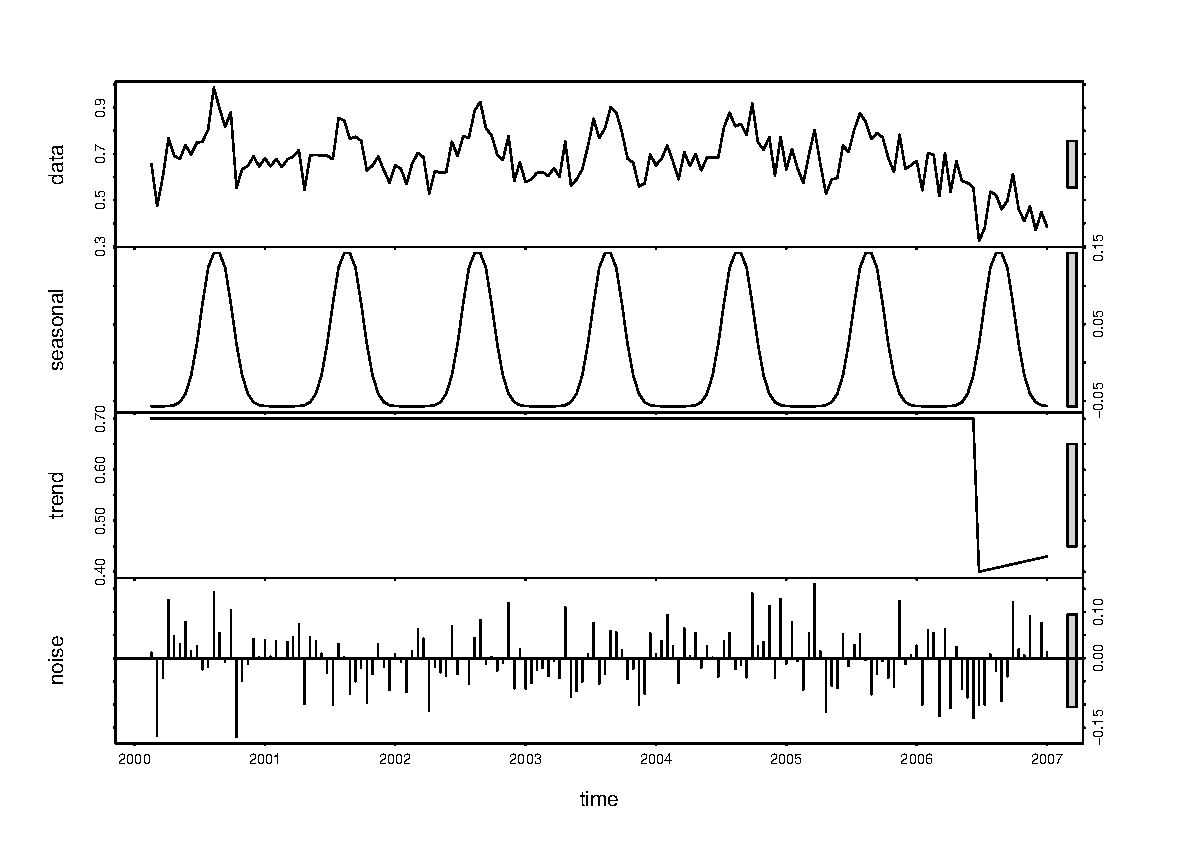
\includegraphics[height=0.7\textwidth]{figs/Sim_Monitoringsetup.eps}
  \caption{Simulated 16-day MODIS NDVI time series (data) with $a$ = 0.2, $\sigma$ = 0.05, containing one simulated abrupt change with $m$ = $-$0.3) (Table~\ref{table:simpar}). The simulated data series is the sum of the simulated seasonal, abrupt and noise series and is used as an input in real-time monitoring method and has a length of 7 years (i.e. 2000--2006) containing a simulated abrupt change in 2006. The solid bars on the right hand side of the plot show the same data range, to aid comparisons.}
  \label{fig:SimSetup}
\end{figure}

\begin{table}[htb]
\caption{Parameter values ($a$, $\sigma$ noise and $m$) for simulation of 16-day NDVI time series while varying the amount of data available in the monitoring period ($n$ i.e. 16-day time steps).}
\centering
\begin{tabular}{ll}
  \hline
  Parameters & Values \\ [0.5ex]
  \hline
  $a$         & $0.1, 0.3, 0.5$ \\
  $\sigma$ noise    & $0.01,0.02,\dots,0.08$ \\
  $m$         & $0, -0.1, -0.2, \dots, -0.5$ \\
  %$\Delta SOS$   & $0, 1.9, 3.2, 4.3$ \\ [.5ex]
  $n$   & $1, 2, \dots, 8$ \\ [.5ex]
  \hline
\end{tabular}
\label{table:simpar}
\end{table}

Two periods within the simulated time series are selected to validate the real-time monitoring approach; (a) a \emph{history period} i.e. data that already has been acquired and which will be analysed for stability in order to model normal vegetation dynamics, and (b) a \emph{monitoring period} i.e. the period representing new data that recently has been captured which needs to be analysed for disturbances. Here, the history is defined as the period from 2000 until mid 2006 (i.e. the time step just before the simulated break), whereas the monitoring period is defined as the period from the simulated break onwards of which the length is gradually increased during the experiment ($n$) (Fig.~\ref{fig:SimMonitor} and Table~\ref{table:simpar}). 

The objective is to verify how much data ($n$) is required before the abrupt change in the monitoring period is detected while varying $\sigma$, $a$, and $m$ (Table~\ref{table:simpar}). The 16-day NDVI time series are simulated by extracting key characteristics from MODIS 16-day NDVI time series within the study area \citep{Verbesselt2009a}. We selected a range of $a$, $\sigma$, and $m$ values for the simulation study to represent a large range of land cover types of different data quality while varying the amount of data available in the monitoring period (Table~\ref{table:simpar}). An example of the set-up of the simulation experiment is shown in Fig.~\ref{fig:SimMonitor}. 1000 iterations of all the combinations of $\sigma$, $a$, $n$ and $m$ were performed to quantify the probability of detecting a disturbance in the monitoring period (i.e. newly acquired data).

%and (2) accuracy of estimating the timing of the detected disturbance change within a time series expressed as Root Mean Square Error (RMSE). 

 \begin{figure}[htp]
\centering
    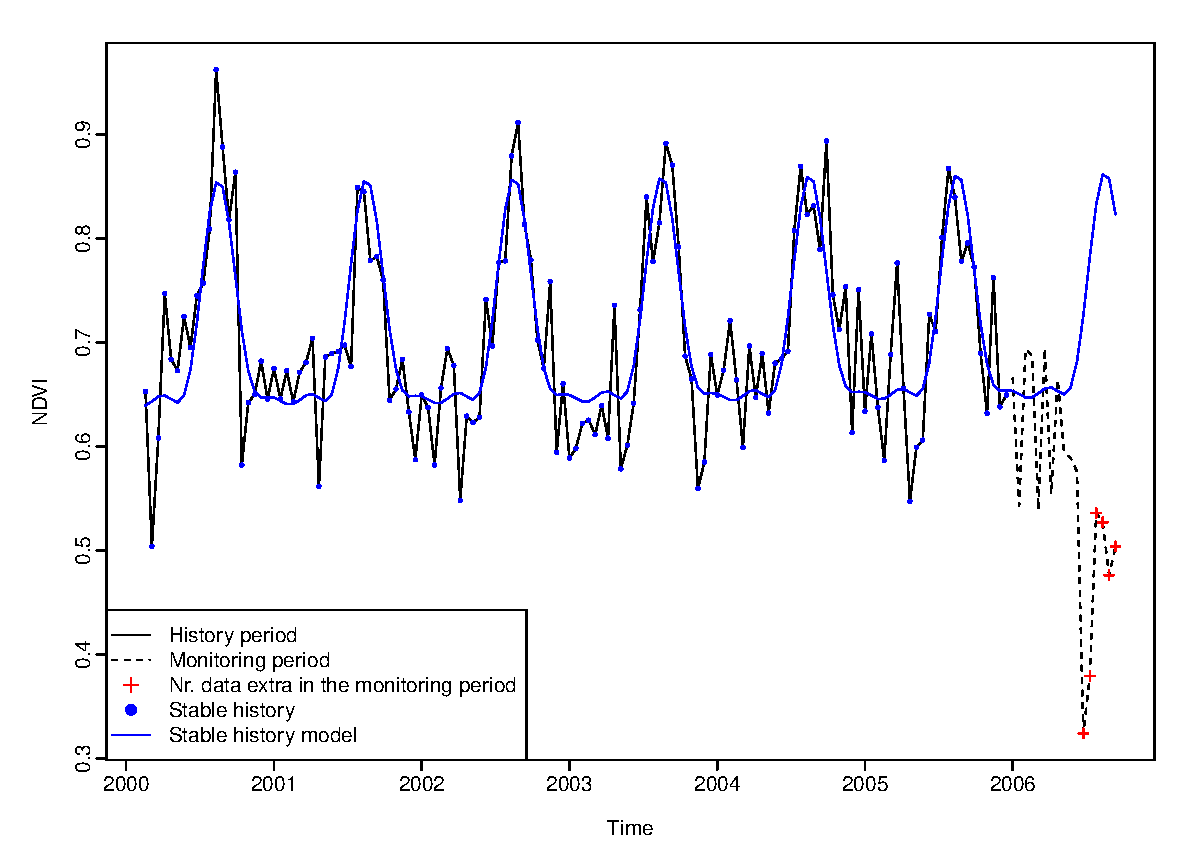
\includegraphics[height=0.5\textwidth]{figs/Sim_Monitoring.eps}
  \caption{Simulated 16-day MODIS NDVI time series with $a$ = 0.2, $\sigma$ = 0.05, containing one simulated abrupt change with $m$ = $-$0.3) (Fig.~\ref{fig:SimMonitor}). During the simulation experiment the period from 2000 until mid 2006 (i.e. the time step just before the simulated break), is considered the \emph{history period} and the period after the simulated break is the \emph{monitoring period}. In this example, $n$ = 6. The result of applying the monitoring approach on the  simulated NDVI series is also shown. A stable history period is identified within the history period and used to model the normal data variation (i.e. stable history model) and predict normal data variation during monitoring period to enable the change detection (Section~\ref{sec:MonStrucChange}). }
  \label{fig:SimMonitor}
\end{figure}

\subsection{Application on real NDVI time series}\label{sec:RealData}
The potential use of the real-time monitoring approach is demonstrated using real MODIS NDVI satellite image time series. To enable comparison with available in-situ forest inventory data, the period from 2000 until end of 2005 was considered as the history period and the year 2006 as the monitoring period. The timing of the detected abrupt changes in the monitoring period (i.e. 2006) revealed were discussed and interpreted using in-situ forest inventory data and expert knowledge \citep{Stone2008,Verbesselt2009}. The seasonal amplitude and noise level were also estimated to illustrate the performance of the method in relation to the obtained results from the simulation experiment. The noise level is estimated by deriving the standard deviation of the residuals from the fitted seasonal-trend model (Section~\ref{sec:seasontrendmodel}) of the stable history period, whereas the amplitude was estimated as the range of the seasonal component of the fitted model.

We selected the 16-day MODIS NDVI composites with a 250m spatial resolution (MOD13Q1 collection~5), since this product provides frequent information at the spatial scale at which the majority of human-driven land cover changes occur \citep{Townshend1988}. The MOD13Q1 16-day composites were generated using a constrained view angle maximum NDVI value compositing technique \citep{Huete2002}. The MOD13Q1 images were acquired from 24 February 2000 to 14 September 2009 for a multi-purpose forested study area (\emph{Pinus radiata} plantation) in South Eastern Australia (Lat.~35.5$^\circ$~S, Lon.~148.0$^\circ$~E). The abrupt, gradual trend changes and phenological shifts occurring within the MODIS 16-day NDVI time series for this study area are described by \citet{Verbesselt2009a,Verbesselt:2010wo}. We used the binary MODIS Quality Assurance flags to select only cloud-free data of optimal quality. Moreover, a pixel time series was only selected for analysis when it lacked less than 10\% of the data \citep{Beurs2009}. 

%Furthermore, the study area consists out of two very different land cover types, i.e., grasslands and plantations, providing time
%series with a large difference in seasonal amplitudes (i.e., 0.05--0.7 NDVI), ideal for evaluating the effect of the seasonal amplitude on change detection method.

\section{Results}

\subsection{Simulation experiment}

Fig.~\ref{fig:SimNr} illustrates the probability for detecting a break within the monitoring period of a time series (i.e. the newly acquired data) while varying the noise level ($\sigma$), magnitude of simulated disturbance in the monitoring period ($m$) and the amount of data available in the monitoring period ($n$). The seasonal amplitude ($a$) did not influence the probability for break detection and results shown in Fig.~\ref{fig:SimNr}  are valid for the different simulated $a$'s (Table~\ref{table:simpar}). Fig.~\ref{fig:SimNr} furthermore shows that a break with $m = -0.2$ can be detected when noise level ($\sigma$) is smaller than 0.04 and $n = 4$ (i.e. 4 images available).  When the magnitude of the to be detected break is larger (e.g. $m = -0.3$), less data points ($n$) are required in the monitoring period for a similar amount of noise (e.g. $\sigma < 0.04$) in the history period.

%Fig.~\ref{fig:SimRMSE} shows the accuracy of time-of-change estimation (16-day time steps) while varying $n$, $m$, and the noise level.
%illustrate fig 1 and 2 of the simulation analysis. amplitude had no effect - no phenological change was simulated - we wanted to test and demonstrate the method for detecting change in forested ecosystems.

\subsection{Spatial application on real data}

The main purpose of applying the real-time monitoring approach onto real data is to demonstrate how the method can be used in a forested areas. Further testing is required to operationally implement the method for detection of other changes in other ecosystems.

Fig.~\ref{fig:SpatNoise} shows the spatial variation of the noise level ($\sigma$) in the study area. The lower noise levels correspond to the forested area within the boundaries of the Pinus radiata plantation. Higher noise levels occur outside the plantation area and correspond to different grassland types. Grassland are influenced more by rainfall and temperature dynamics which explain a high seasonal amplitude and large phenological shifts (e.g. start and end of the growing season) \citep{Verbesselt:2010wo}, which explains the higher noise levels. Therefore, results in Fig.~\ref{fig:SpatTimeofChange} and Fig.~\ref{fig:SpatLStableHist} are shown for the region within the boundaries of the forest plantation, which approximately corresponds to the lower noise levels in Fig.~\ref{fig:SpatNoise} and noise range used in the simulation experiment (Table~\ref{table:simpar} and Fig.~\ref{fig:SimNr}).

Fig.~\ref{fig:SpatTimeofChange} illustrates the time of the detected changes within 2006. Many changes are detected in 2006 due to a drought that occurred around that time in combination with harvest operations. Fig.~\ref{fig:SpatLStableHist} shows the length of the stable history period (years) and illustrates where recent changes occurred in the history period (e.g. a recent harvest operation). Fig.~\ref{fig:realmonitoring} and Fig.~\ref{fig:shorthistory} are examples for specific location in the study area illustrating what the length of the history period is, and when and how a change is detected in the history period. The drought stress is the main driver of the disturbance detected in the top graph of Fig.~\ref{fig:realmonitoring} whereas a harvest operations explain the change detected in the bottom graph of Fig.~\ref{fig:realmonitoring}. A different length of the automatically identified stable history is also visible. Another drought event in 2003 potentially can explain the shorter stable history identified in Fig.~\ref{fig:realmonitoring} (top) while the the full history period was considered as stable in Fig.~\ref{fig:realmonitoring} (bottom). Tthe noise level in the time series is a little higher combined with the fact that the drougth has smaller impact on the seasonal NDVI dynamics (Fig.~\ref{fig:realmonitoring} (bottom)).

Fig.~\ref{fig:shorthistory} shows an example of harvests operation which is occurring in the history period and explain why a shorter history period is being detected. A change is still detected in 2006 because harvest operation was still occurring at that time.

% the length of the stable history period could be used the restrict analysis to specific regions.

% create a raster with gids and then export that rasters so that we can query pixels and look at the data to further understand the results.
% WAT IS THE EFFECT OF THE STABLE HISTORY LENGTH ON THE PROBABILITY OF CHANCE DETECTION?

\section{Discussion and further work}

While the data and methods used here are appropriate for proof-of-concept development, other applications (e.g. deforestation monitoring or oil spill detection) will mandate further calibration and validation and use-specific remote sensing platforms \citep{White2006}, as discussed below.

1. data set selection - daily? - cloud effect discussion - sentinel or the dmc constellation - this analysis was done using 16-day data however in operational situation daily data could be used - further testing needs to be done to verify how this method can be optimized to handle daily data which potentially is more noise.

% modis rapid response, meteosat geostationary satellites, etc.

2. phenological change detection is also possible. 
Continuous modelling of the seasonality using the proposed concept also allows for relateing remote sensing to a continual process of land surface phenology change instead of a single date extraction \citep{Verbesselt:2010wo,White2006}

Ideal prediction period discussion:
(1) how much data is needed before a break can be detected? 
(2) how much data can be used before the prediction of the model is not valid anymore?.  . See forecasting papers and also White et al. paper.

3. Pro's and con's of data simulation. Data simulation enables testing of a method however with data simulation it is very difficult to reproduce similar behavior as in real time series e.g. measured by satellite sensors of vegetation dynamcis.
Further work

4. no decompositioning is done here - one model is being used.

5. monitoring should be exported in an area where you now that the history period is more or less stable. e.g. if deforestation has happend in the year before the monitoring period than it should not be exported but been masked out from the analysis for example.

6. also keep in mind that positive and negative change are being detected so we should in a further fase verify in which coefficients (beta) of the most of the changes occur.

7. keep in mind that if there is a regrowth effect occurring and the ndvi is saturising we are detecting a change while in reality there is no real change.

The real-time monitoring could be further improved by including other explanatory variables in the monitoring model (e.g. temperature, rainfall) which will contribute to model the data and determine what is normal versus what is abnormal. Furthermore, the monitoring model proposed here can also further improved to be used as a forecasting model. Similar to current real-time monitoring approach, forecasting requires a profound understanding of vegetation dynamics and vegetation interaction with the atmosphere, combined with proper data analysis techniques  \citep{LeiJi:2004kx}.


8. no data gaps are filled - see e-mail of Achim!
%More info for other applications of this methodology:
%\url{http://rapidfire.sci.gsfc.nasa.gov/} 
% This might be an interesting link for real time change detection and application if we really want to detect changes fast
% if we really want to detect changes in real-time we should use the MODIS rapid response option
% this certainly needs to be mentioned in the discussion -- 


% for testing the method we will use 16-day MODIS time series for fit a normal seasonal change pattern (monitoring the stable period) and potentially use daily images to do the abrupt monitoring? or should we stick to the 16-day image at the end of the time series (easier!!! for programming purposes).

\readme{Deviations from �normal� land surface phenologi- cal development can be the first indications of important changes in forest health, including disturbance and recovery (de Beurs and Henebry 2005, Liang and Schwartz 2009, Morisette et al. 2009), carbon status, and even climatic shifts (Cleland et al. 2007).}

!!!!
\readme{
Further, many methods assume that a given mathematical func- tion, such as piecewise logistic functions (Zhang et al., 2003), approximates true phenological development. In global, or even regional application this may be an untenable assumption, es- pecially in cases of disturbance, defoliation, or NDVI curves with sharp peaks or broad plateaus (Potter et al., 2003).}


\readme{adding co-variates e.g. like temperature, precipitation might help differentiating a real change from seasonality.}


\section{Conclusion}
Currently, real-time satellite images and their derivatives are routinely produced and published on the World wide Web (e.g. \url{http://rapidfire.sci.gsfc.nasa.gov/} or \url{http://www.dmcii.com/index.html}) but methods for real-time monitoring and change detection are lacking. 

the method can be used for meteorological satellites - which provide real-time data - e.g. monitoring of evapotranspiration or NEP, NPP, carbon dynamics in real-time.

The method is a fast, and simple method which easily can be applied onto other remotely sensed data sets. Further testing is certainly to validate it in other ecosystems (e.g. grasslands or agricultural fields).


This validation approach by combining tests with simulated and real data should be a standard practice when validating novel change detection approaches. Furthermore, methods being proposed should also be made available to other scientist enabling the reproducibility of the research and collaboration towards further improvement of the methods.


%The approach is adaptable to different remote sensing technologies and provides a foundation for ascribing a sequence of ground conditions (e.g. snowmelt, vegetative growth, pollen production, insect phenology) to remotely sensed land surface phenology observations \citep{White2006}.

\section{Acknowledgements}

This work was undertaken using expertise and field data available via the program of the Cooperative Research Center for Forestry: Monitoring and Measuring (\url{http://www.crcforestry.com.au}). Marie Curie !!! Number of my grant?

%Thanks to xx whose comments greatly improved this paper. We greatly appreciate the constructive feedback we have received from the three reviewers.


\bibliographystyle{model5-names}
\bibliography{refs}

\newpage

\section*{Figures}

 (For interpretation of the references to color in this figure legend, the reader is referred to the web
 version of this article.)

\begin{figure}[htp]
\centering
    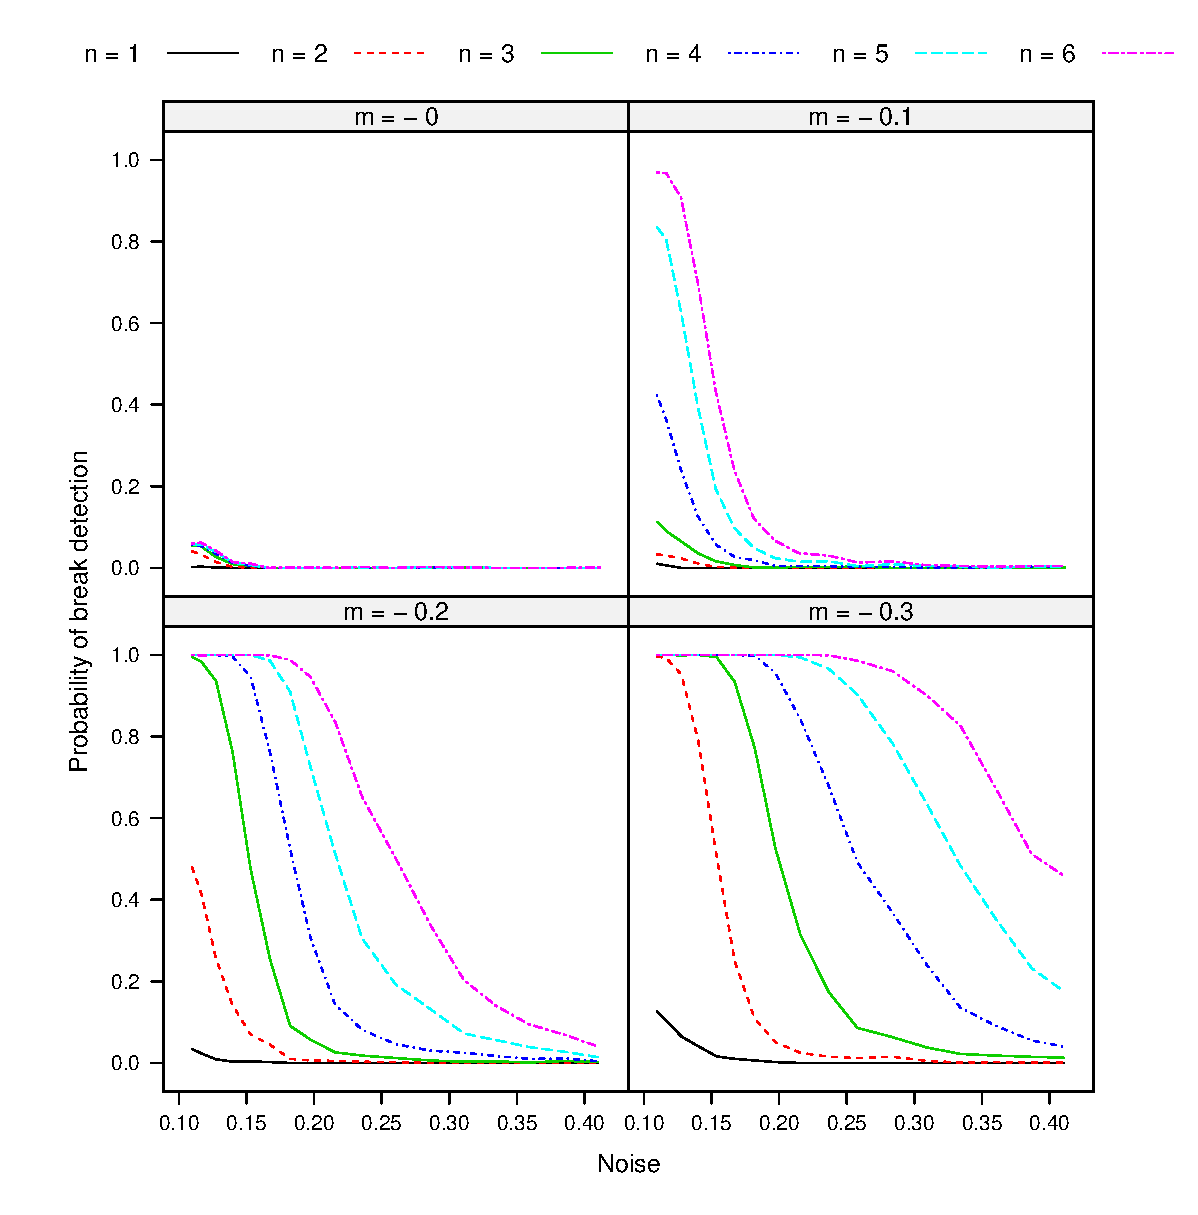
\includegraphics[height=0.9\textwidth]{figs/NrDetections_Time_1000.eps}
  \caption{Results from the simulation experiment (1000 iterations) illustrating the probability for break detection in the monitoring period while varying the amount of noise ($\sigma$), magnitude of the simulated break ($m$), and amount of data  available in the monitoring period ($n$). The units of the x and y-axis are noise (i.e. $\sigma$ NDVI of the residuals of the fitted seasonal-trend model on the history period) and probability of detecting a break (i.e. proportion of detected breaks in 1000 iterations). See description of the simulation experiment for more details (Section \ref{sec:Valsim}). }
  \label{fig:SimNr}
\end{figure}

%\begin{figure}[htp]
%\centering
%    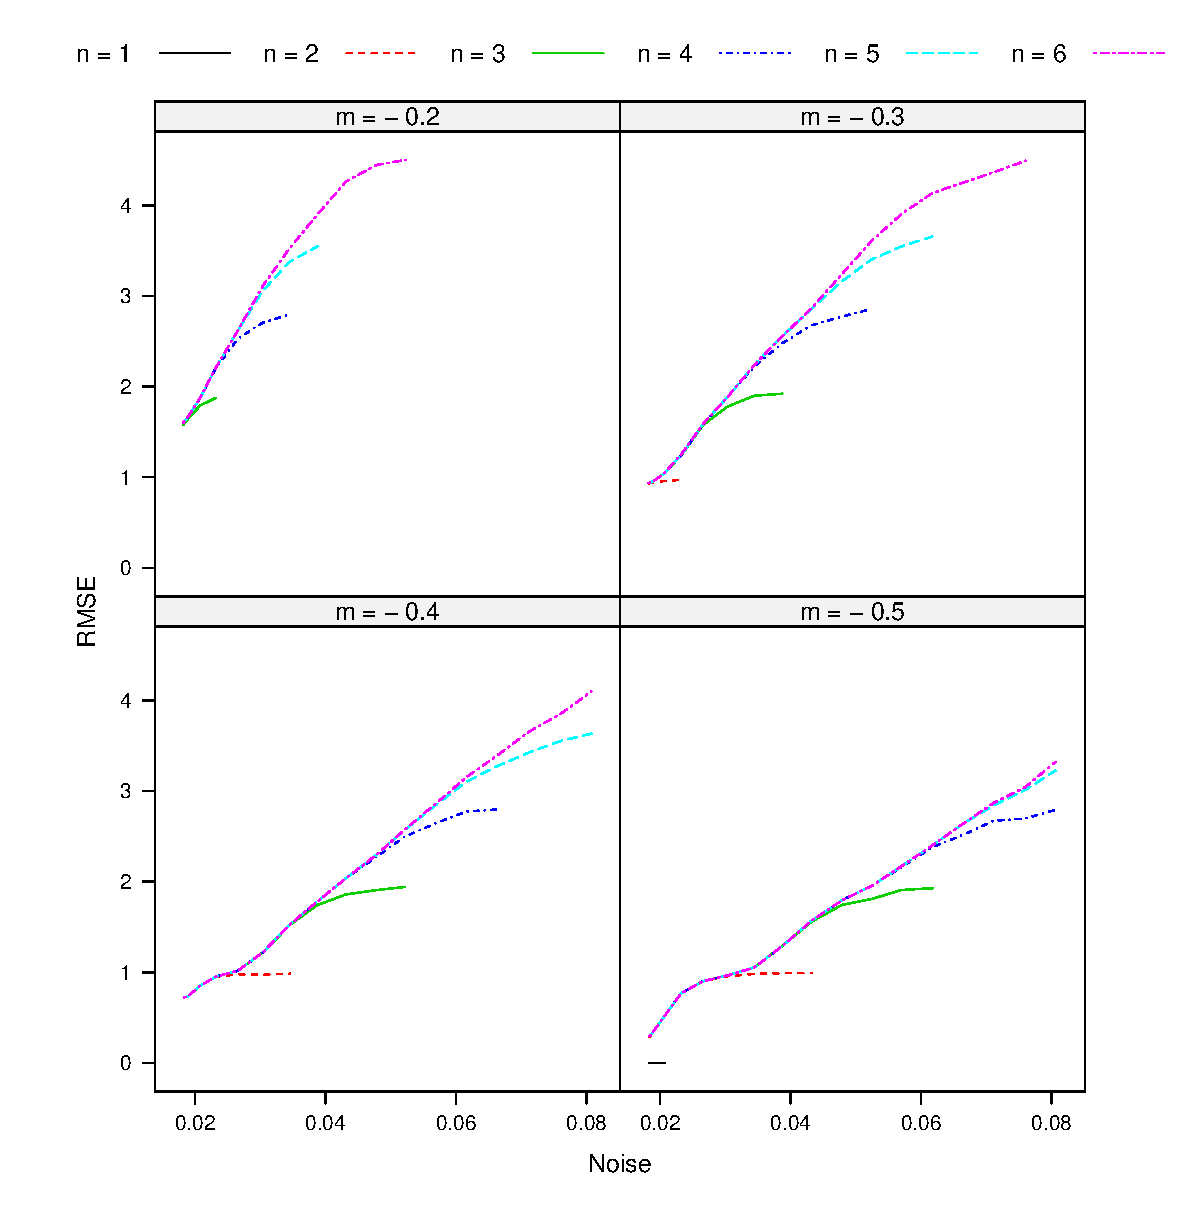
\includegraphics[height=0.9\textwidth]{figs/RMSE_Time_1000.eps}
%  \caption{Results from the simulation experiment (1000 iterations) illustrating the accuracy of time estimation of the detected breaks while varying the amount of noise, magnitude of simulated break ($m$), and amount of data available in the monitoring period ($n$). The units of the x and y-axis are noise (i.e. noise range expressed in NDVI) and RMSE (i.e. time steps between images where 1 equals a 16-day period). See description of the simulation experiment for more details (Section \ref{sec:Valsim}).}
%  \label{fig:SimRMSE}
%\end{figure}

%\begin{figure}[htp]
%\centering
%    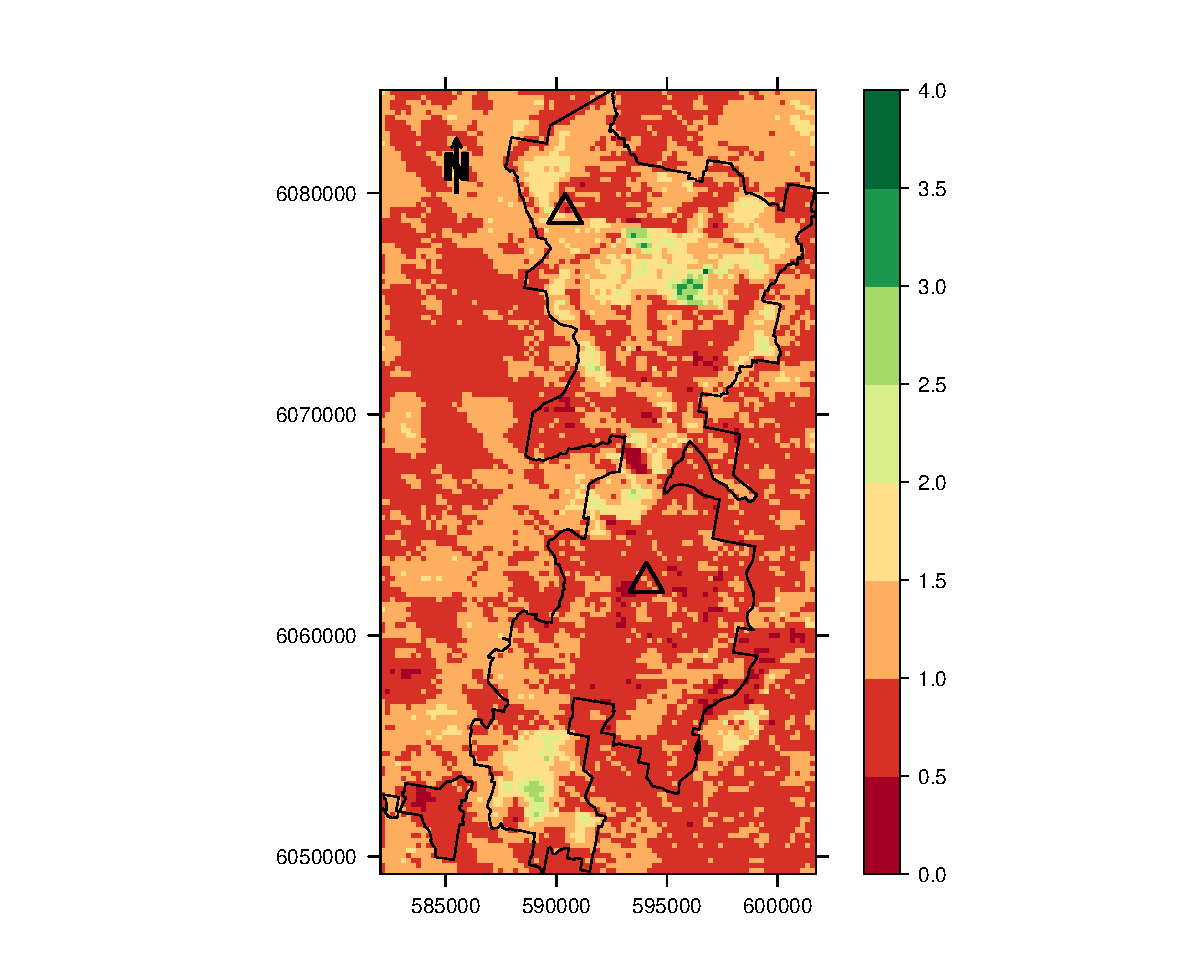
\includegraphics[height=0.9\textwidth]{figs/SignaltoNoiseRatio.eps}
%  \caption{Spatial variation of the signal to noise ratio is the study area. (Try out: only for your information - not sure whether I will include this in the paper) }
%  \label{fig:SpatSignalNoise}
%\end{figure}

\begin{figure}[htp]
\centering
    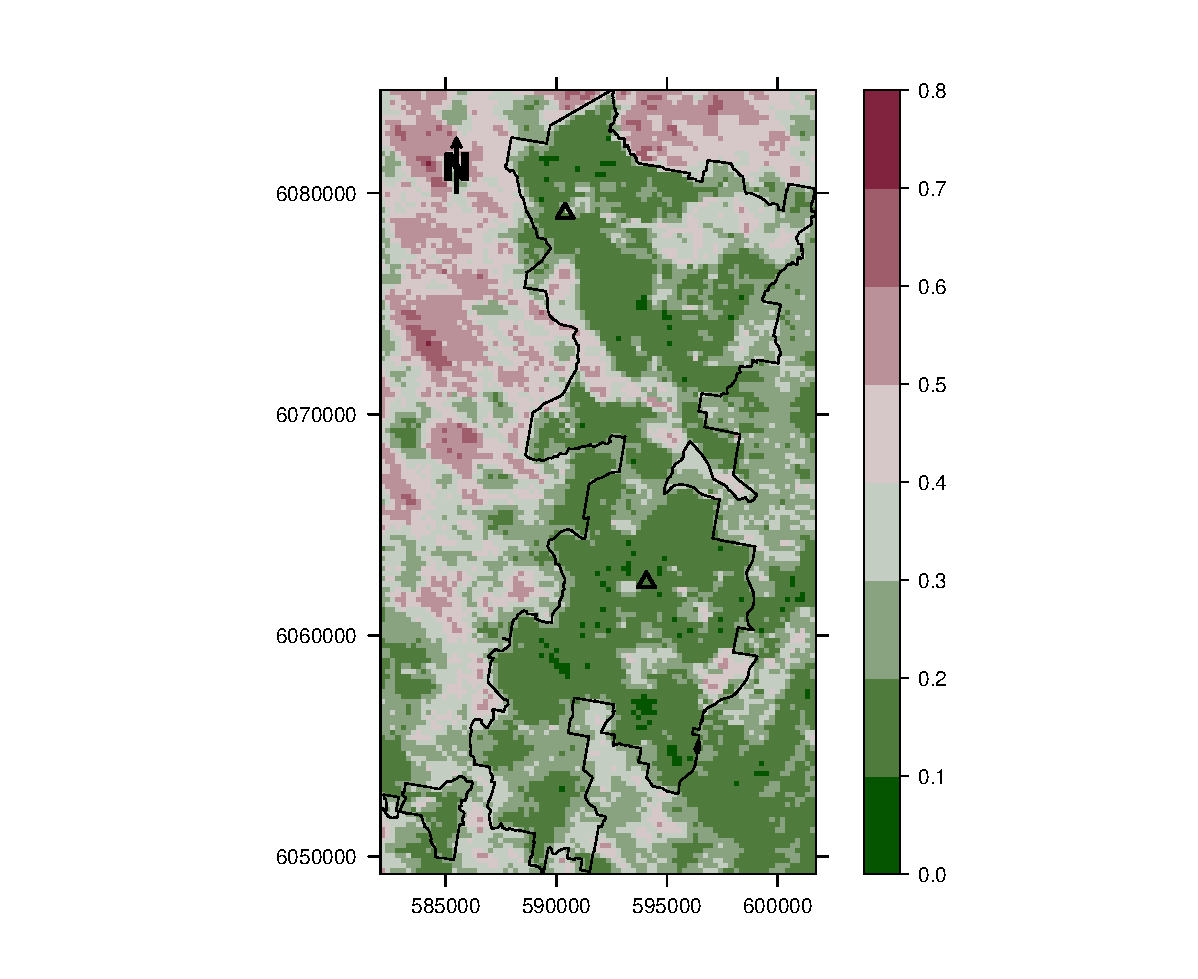
\includegraphics[height=0.9\textwidth]{figs/Noise.eps}
  \caption{Spatial variation of the noise level (i.e. the standard deviation of the residuals of the stable history model) in the study area, a forested area in south eastern Australia. The black line indicates the boundary of the Pinus radiata plantation, which corresponds to the area with a lower noise level. The plantation is surrounded by grasslands.}
  \label{fig:SpatNoise}
\end{figure}

\begin{figure}[htp]
\centering
    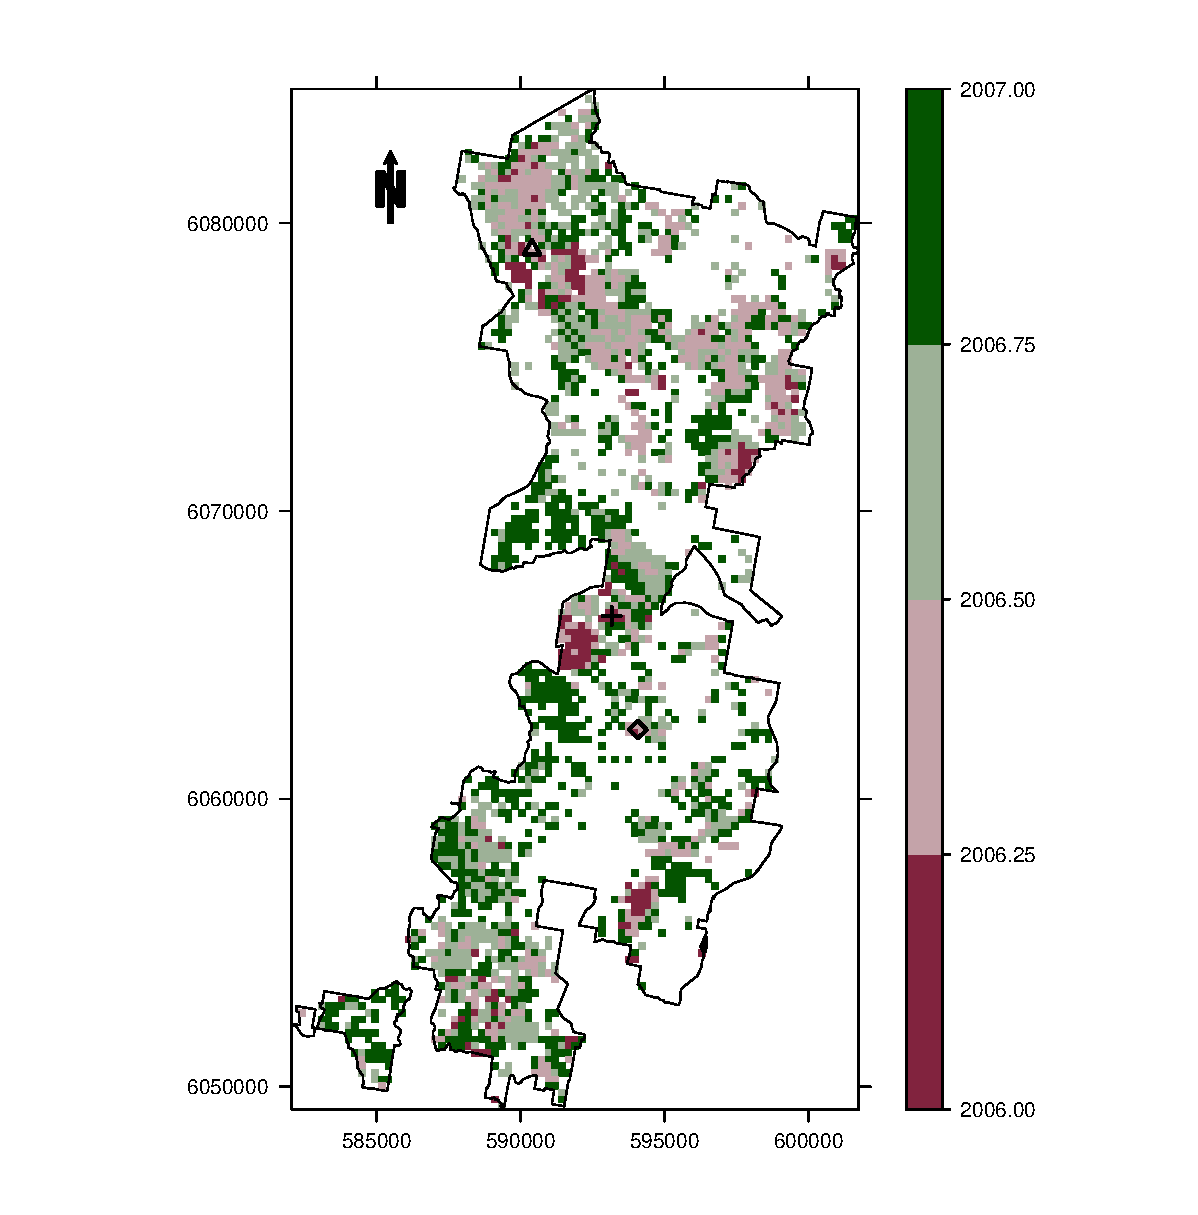
\includegraphics[height=0.9\textwidth]{figs/TimeofChangein2006_II.eps}
  \caption{Time of detected changes within the study area in the monitoring period (i.e. 2006), where white indicates that no change is detected for a forested area in south eastern Australia. The black line indicates the boundary of the Pinus radiata plantation which is surrounded by grasslands.}
  \label{fig:SpatTimeofChange}
\end{figure}

\begin{figure}[htp]
\centering
    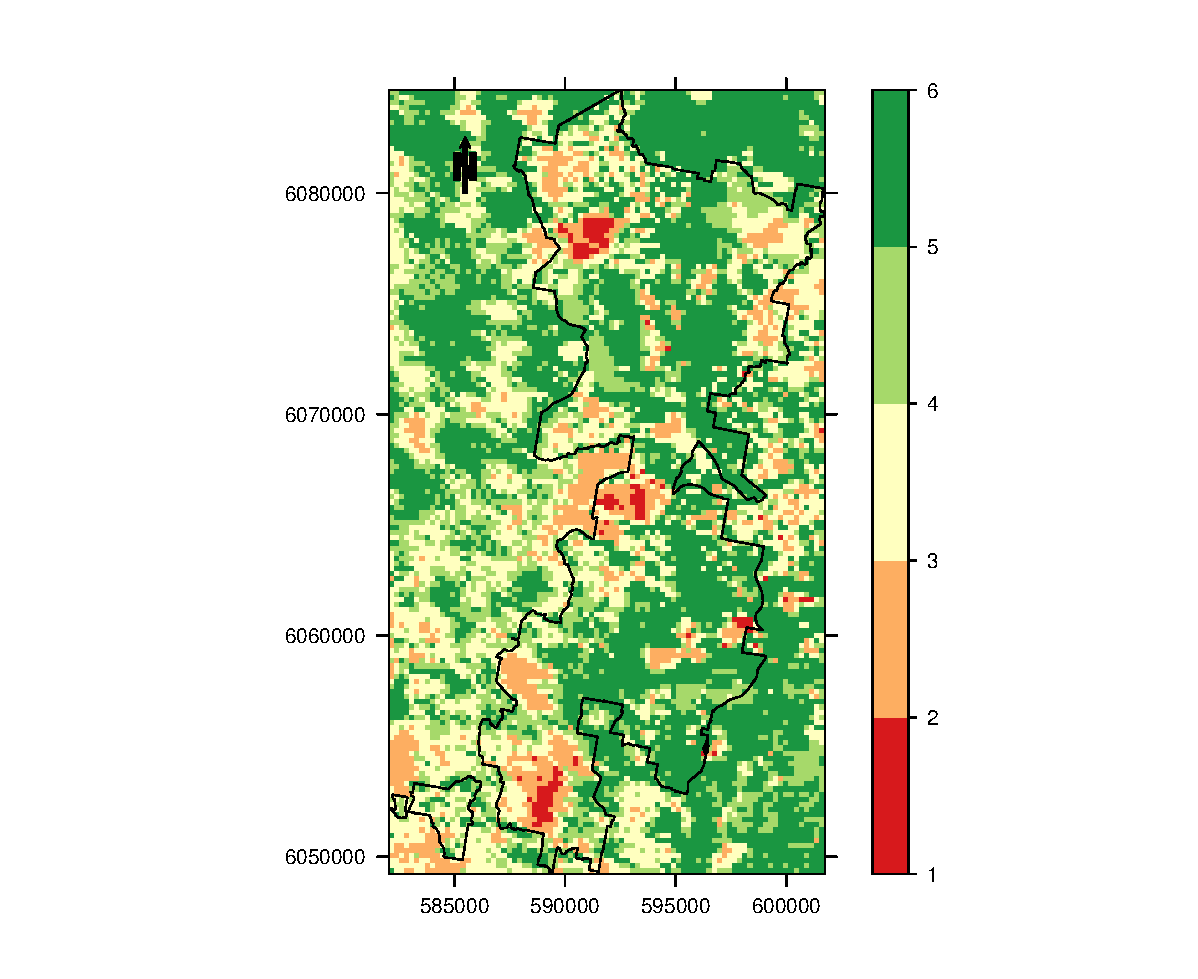
\includegraphics[height=0.9\textwidth]{figs/LengthStableHistory.eps}
  \caption{Spatial variation of the length the stable history period (expressed in years, i.e. 23 16-day images) of a forested area in south eastern Australia. The black line indicates the boundary of the Pinus radiata plantation, which is surrounded by grasslands. The length of the history period indicates when in the history period a potential disturbance occurred (e.g. shorter length indicates a more recent disturbance). }
  \label{fig:SpatLStableHist}
\end{figure}

\begin{figure}[htp]
\centering
    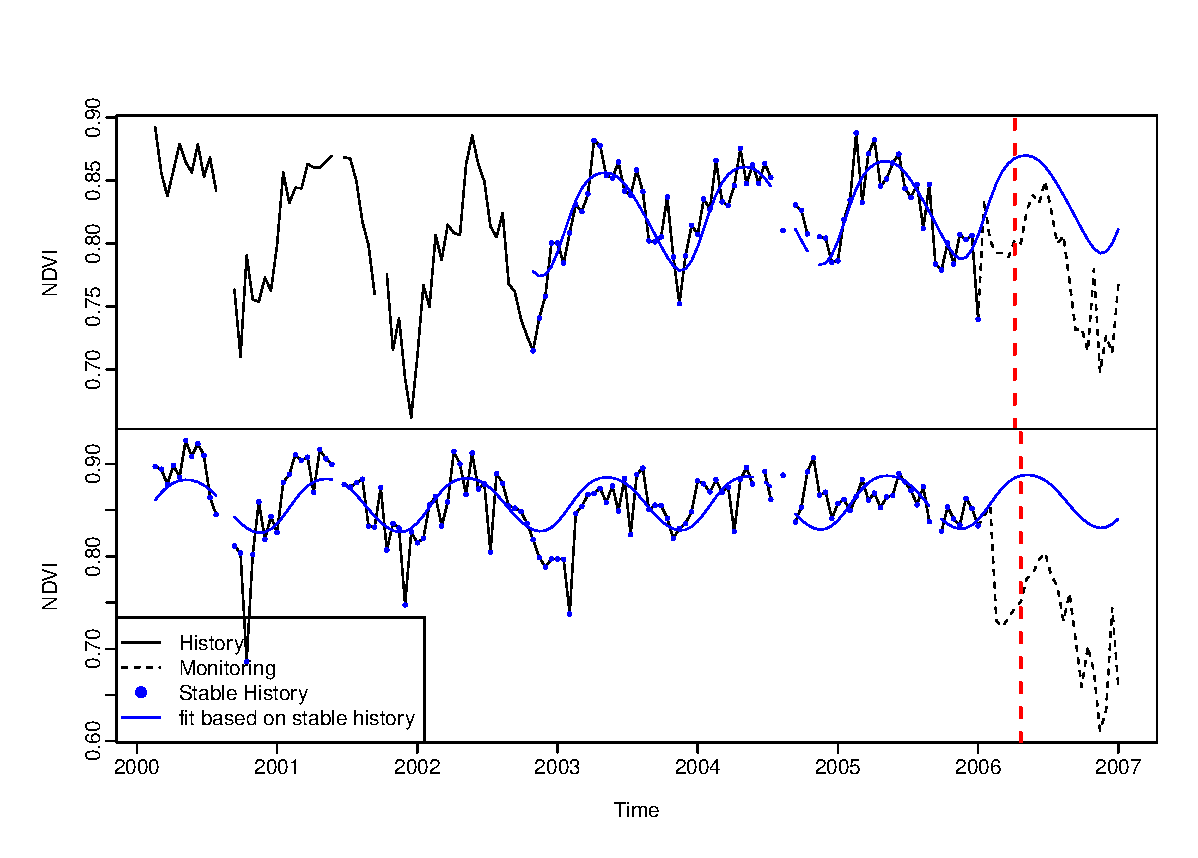
\includegraphics[height=0.6\textwidth]{figs/realmonitoring.eps}
  \caption{
  %plot 120 and 8
  Results of real-time monitoring approach applied onto 16-day MODIS NDVI time series for two locations, i.e. $\diamondsuit$ (top) and $\triangle$ (bottom) on Fig.~\ref{fig:SpatNoise}, \ref{fig:SpatTimeofChange} and \ref{fig:SpatLStableHist}), situated within the Green Hills study area. In both time series a break (vertical red dashed line in 2006) is detected in the monitoring period (i.e. 2006) while using 2000 until end of 2005 as a history period. A stable history period (blue dots) is automatically detected with the history period. The method is able to deal with time series with data gaps (e.g. after cloud removal) which is illustrated by data gaps within the data analyzed and model fit based on the stable history period.}
  \label{fig:realmonitoring}
\end{figure}

\begin{figure}[htp]
\centering
    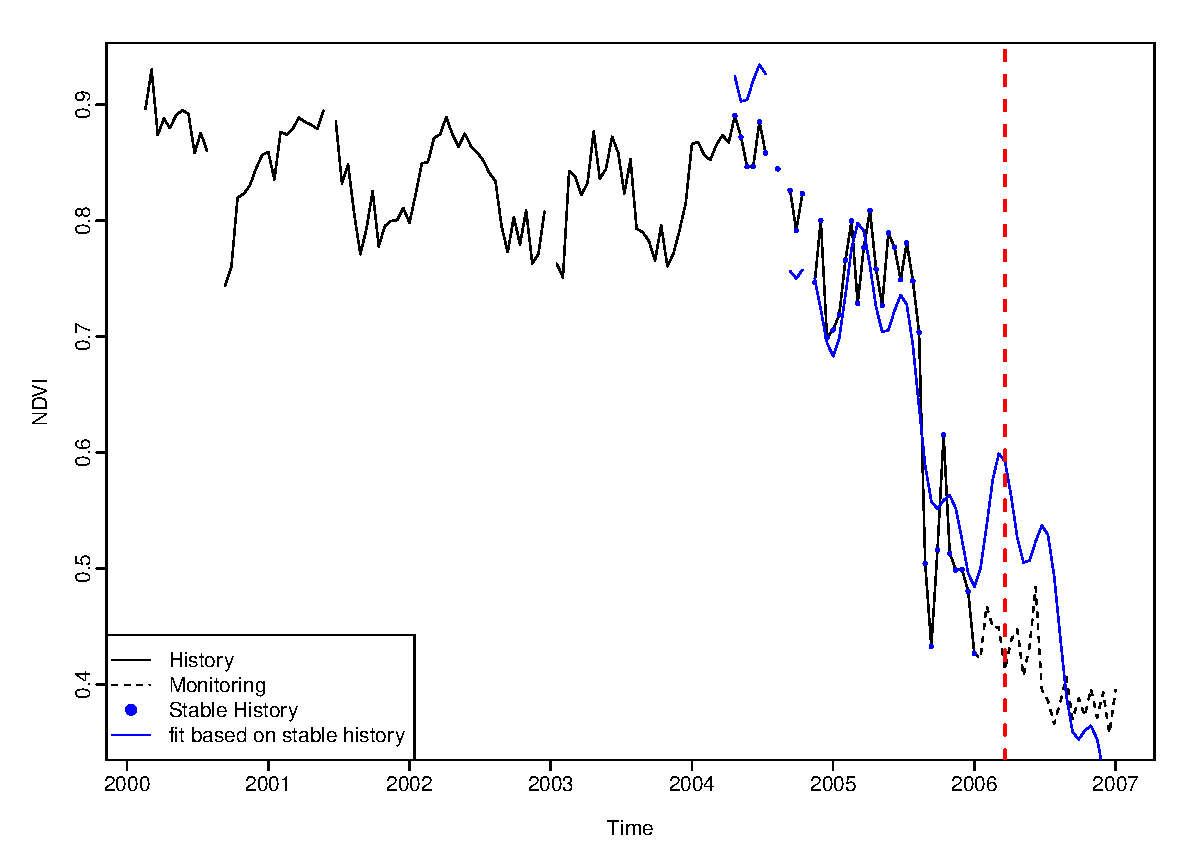
\includegraphics[height=0.6\textwidth]{figs/shorthistoryperiod.eps}
  \caption{
  Results of real-time monitoring approach applied onto 16-day MODIS NDVI time series for a location situated within the Green Hills study area (i.e. the $+$ symbol on Fig.~\ref{fig:SpatNoise}, \ref{fig:SpatTimeofChange} and \ref{fig:SpatLStableHist}) . A break (vertical red dashed line in 2006) is detected in the monitoring period (i.e. 2006) while using 2000 until end of 2005 as a history period. A short stable history period (blue dots) is detected within the history period due to an ongoing harvest operation. The method is able to deal with time series with data gaps (e.g. after cloud removal) which is illustrated by data gaps within the data analyzed and model fit based on the stable history period.}
  \label{fig:shorthistory}
\end{figure}

%\begin{figure}[htp]
%\centering
%    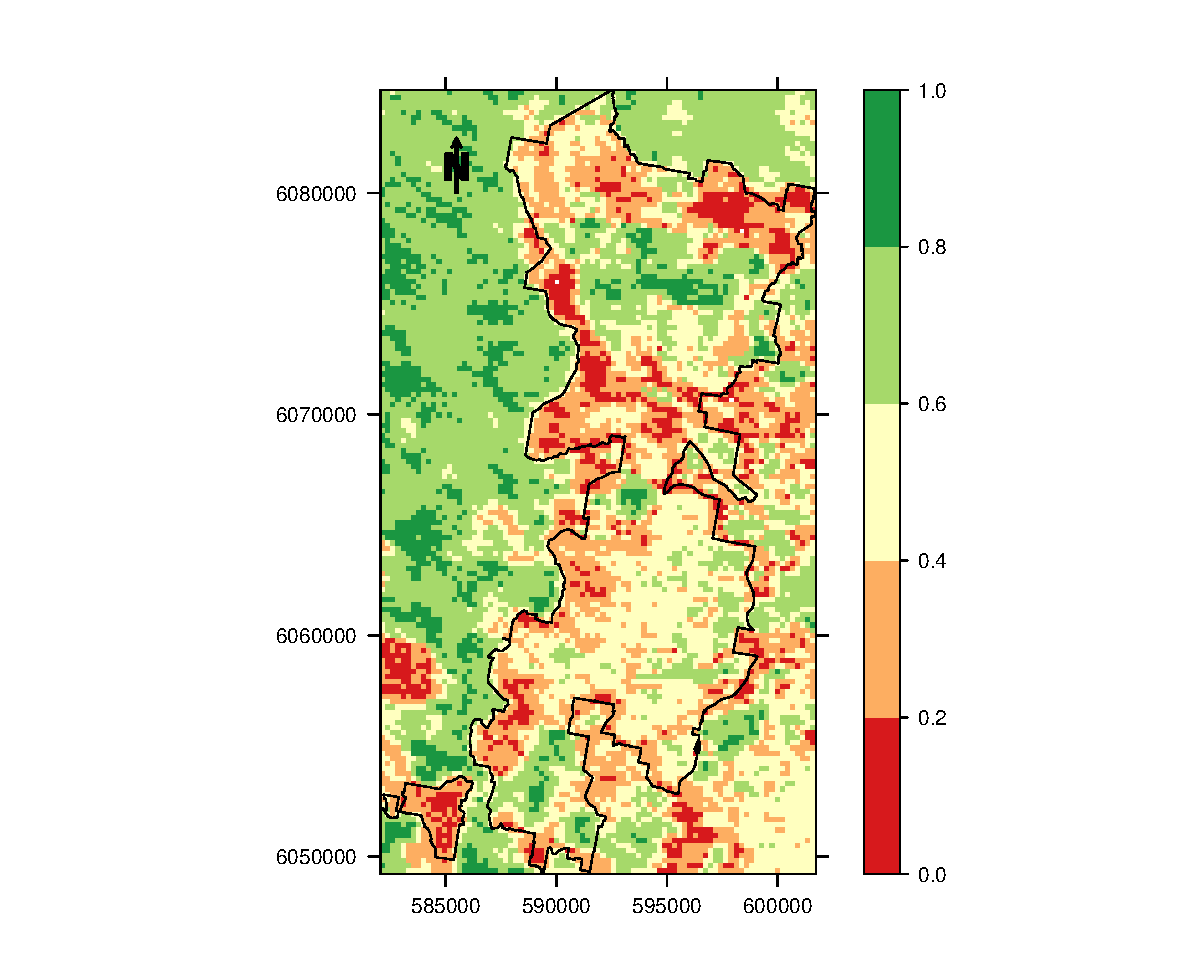
\includegraphics[height=0.9\textwidth]{figs/R2ofthemodelfit.eps}
%  \caption{ Spatial variation of the $R^2$ of the model fit which also depend on the length the stable history period}
%  \label{fig:SpateR2}
%\end{figure}

\end{document}

